% ============================================================
%  AI vs Real Image Detection: A Multi-Branch Tandem Study
%  Two-column ACL / IEEE-style paper
%  Compile with: pdflatex -> bibtex -> pdflatex x2
% ============================================================
\documentclass[10pt,twocolumn]{article}

% ── Packages ────────────────────────────────────────────────
\usepackage[margin=1in,top=0.8in,bottom=0.8in]{geometry}
\usepackage{times}
\usepackage{latexsym}
\usepackage{amsmath,amssymb}
\usepackage{graphicx}
\usepackage{booktabs}
\usepackage{multirow}
\usepackage{array}
\usepackage{tabularx}
\usepackage{url}
\usepackage{hyperref}
\usepackage{xcolor}
\usepackage{caption}
\usepackage{subcaption}
\usepackage{enumitem}
\usepackage{microtype}
\usepackage{titlesec}
\usepackage{abstract}
\usepackage[numbers,sort&compress]{natbib}
\usepackage{tikz}
\usetikzlibrary{shapes.geometric, arrows.meta, positioning, fit, backgrounds}

% ── TikZ styles for architecture diagrams ───────────────────
\tikzstyle{block} = [rectangle, rounded corners=3pt,
    minimum width=3.2cm, minimum height=0.55cm,
    text centered, draw=black, font=\footnotesize,
    inner sep=3pt]
\tikzstyle{cnnblock}  = [block, fill=violet!20]
\tikzstyle{texblock}  = [block, fill=orange!20]
\tikzstyle{fusblock}  = [block, fill=teal!20]
\tikzstyle{lossblock} = [block, fill=red!20]
\tikzstyle{arrow}     = [-{Stealth[length=5pt]}, thick]
\tikzstyle{dasharrow} = [-{Stealth[length=5pt]}, dashed, thick, gray]

% ── Title formatting ─────────────────────────────────────────
\titleformat{\section}{\normalfont\large\bfseries}{\thesection}{0.6em}{}
\titleformat{\subsection}{\normalfont\normalsize\bfseries}{\thesubsection}{0.5em}{}
\titleformat{\subsubsection}{\normalfont\normalsize\itshape}{\thesubsubsection}{0.5em}{}
\setlength{\columnsep}{0.3in}

% ── Hyperref colours ─────────────────────────────────────────
\hypersetup{colorlinks=true, linkcolor=blue!70!black,
            citecolor=blue!70!black, urlcolor=blue!70!black}

% ============================================================
\begin{document}

% ── Title block ─────────────────────────────────────────────
\twocolumn[{%
\begin{center}
{\LARGE\bfseries Detecting AI-Generated Images via\\
Multi-Branch Feature Fusion: A Tandem Study of\\
Texture, Forensic, and Contrastive Objectives\par}
\vspace{0.8em}
{\large Anonymous Authors\par}
\vspace{0.2em}
{\normalsize Image Processing \& Pattern Recognition Course Project\par}
\vspace{0.8em}
\end{center}
\begin{abstract}
\noindent
The rapid proliferation of photo-realistic generative models demands
robust detectors that go beyond simple visual cues.
We present a systematic study of five CNN-based classifiers for
binary \emph{Real vs.\ AI-Generated} image detection on the
\textsc{ShreyashDhoot/AI\_vs\_Real} dataset (\textasciitilde180\,K images,
1.49:1 class imbalance).
Starting from a plain deep CNN baseline trained with Binary Cross-Entropy (BCE),
we progressively introduce (i) residual connections and Focal Loss, and
then propose three \emph{tandem} architectures that fuse a
CNN visual branch with a 96-dimensional Gray-Level Co-occurrence Matrix
(GLCM) texture branch and an 8-dimensional forensic gradient/residual branch.
Two auxiliary objectives---patch-view KL consistency and supervised
contrastive loss---are further evaluated atop the tandem baseline.
Our best single model (Tandem-Baseline) achieves
\textbf{F1\,=\,0.762}, \textbf{ROC-AUC\,=\,0.791}, and
\textbf{PR-AUC\,=\,0.768} on a class-balanced 250-sample test split,
while the Focal-Loss CNN reaches \textbf{F1\,=\,0.714},
\textbf{ROC-AUC\,=\,0.802} on the full 18\,K test set.
We analyse the impact of each design choice, present a comparative
literature survey, and outline the novel aspects of our contributions
relative to contemporary detection methods.
\end{abstract}
\vspace{1em}
}]

% ============================================================
\section{Introduction}
\label{sec:intro}

Generative Adversarial Networks (GANs)~\cite{goodfellow2014generative}
and Diffusion Models~\cite{rombach2022ldm} now produce imagery that is
visually indistinguishable from real photographs for human observers.
This capability, while enabling creative applications, has simultaneously
fuelled a surge in AI-related fraud, disinformation campaigns, and
identity manipulation~\cite{tasnim2025empirical}.
Market projections suggest generative-AI fraud losses could approach
\$40\,billion annually by 2027, with deepfake-related cryptocurrency
scams increasing 456\% between May 2024 and April
2025~\cite{tasnim2025empirical}.

Detecting AI-generated images is therefore an urgent forensic problem.
Early methods relied on hand-crafted spatial-domain cues such as colour
statistics, saturation anomalies, or JPEG compression traces
\cite{wang2020cnns}, but these struggle to generalise as generators evolve.
Modern approaches span CNN-based classifiers~\cite{wang2020cnns},
frequency-domain analysis~\cite{frank2020leveraging},
texture-feature fusion~\cite{liu2020gram,frontiers2025multimodal},
and contrastive or language-guided representation
learning~\cite{wu2023lasted,hong2024contrastive}.
Transformers~\cite{lamichhane2025vit} and CLIP-based
zero-shot detectors~\cite{ojha2023universal} mark the current frontier,
yet compact, interpretable models trained from scratch on moderately
sized, class-imbalanced corpora remain understudied.

Our work addresses this gap.
Concretely, we make the following contributions:
\begin{enumerate}[leftmargin=*, noitemsep]
  \item A thorough empirical comparison of \textbf{five architectures}
        spanning plain CNNs to multi-branch tandem models on a single
        real-world dataset with controlled evaluation protocol.
  \item A novel \textbf{three-branch tandem design} that fuses CNN visual
        features with handcrafted GLCM texture statistics and forensic
        gradient/residual features---a combination not previously studied
        in this joint formulation.
  \item Systematic evaluation of \textbf{two auxiliary objectives}
        (patch-view KL consistency and supervised contrastive loss)
        applied to fused multi-branch representations.
  \item Analysis of \textbf{Focal Loss with threshold tuning} as a
        principled approach to imbalanced forensic classification,
        showing a +15.4\% recall and +9.1\% F1 gain over BCE.
\end{enumerate}

% ============================================================
\section{Related Work}
\label{sec:related}

\subsection{CNN-Based Detectors}

Wang~et~al.~\cite{wang2020cnns} showed that a ResNet-50 trained
only on ProGAN outputs transfers surprisingly well to other GAN
architectures, establishing the CNN classifier as a strong baseline.
Subsequent work by Tan~et~al.~\cite{tan2024npr} on Neighboring Pixel
Relationships (NPR) extended this by capturing upsampling traces
inherent to generative pipelines, and Liu~et~al.~\cite{liu2024fatf}
introduced frequency-aware adapters via forgery-aware transformers.
Our \textbf{Basic CNN} and \textbf{Focal-Loss CNN} sit in this
family---scratch-trained, four-block residual classifiers with
progressive dropout and L2 regularisation.

\subsection{Texture and Frequency Features}

Handcrafted descriptors remain competitive in low-data regimes.
Liu~et~al.~\cite{liu2020gram} (Gram-Net) demonstrated at CVPR\,2020 that
GLCM contrast statistics differ measurably between real and GAN-generated
faces across spatial distances.
Frontiers~\cite{frontiers2025multimodal} very recently proposed a
multi-modal fusion network that explicitly incorporates GLCM and LBP
channels alongside RGB, achieving strong generalisation across GAN and
diffusion-model outputs.
Frank~et~al.~\cite{frank2020leveraging} used DCT spectral analysis
to expose periodic upsampling artefacts in frequency space.
Our tandem architecture is aligned with the GLCM-fusion spirit
of~\cite{frontiers2025multimodal} but extends it with a dedicated
\emph{forensic} branch capturing gradient PCA and noise residual
statistics---a combination not present in prior work.

\subsection{Contrastive and Self-Supervised Approaches}

Contrastive learning has been applied to forgery detection to improve
feature separability~\cite{wu2023lasted,hong2024contrastive,
niloy2023cfl,gu2022hierarchical}.
Wu~et~al.~\cite{wu2023lasted} (LASTED) leveraged language-guided
contrastive supervision with CLIP for cross-generator generalisation.
Hong~et~al.~\cite{hong2024contrastive} applied multi-label ranking
with contrastive objectives for deepfake localisation.
Our \textbf{Tandem-Contrast} model applies supervised contrastive
loss~\cite{khosla2020supervised} at temperature $\tau=0.07$ directly
on the projected fused features---a compact alternative that avoids
large pre-trained encoders.

\subsection{Focal Loss for Imbalanced Detection}

Lin~et~al.~\cite{lin2017focal} introduced Focal Loss to down-weight
easy negatives in dense object detection.
Its use for imbalanced forensic classification is less
explored; we provide a detailed empirical comparison demonstrating its
advantages over BCE for the specific 1.49:1 class imbalance
encountered in our dataset.

\subsection{Patch-Based Consistency}

PatchCraft~\cite{zhong2023patchcraft} exploits texture discrepancy
between rich- and poor-texture patches for AI detection.
Our \textbf{Tandem-Patch} model is related in spirit: it enforces KL
consistency between two random patch crops of the same image,
encouraging the model to produce stable predictions under local view
perturbation---a form of self-supervised regularisation not previously
combined with GLCM fusion in this context.

% ============================================================
\section{Dataset and Problem Setting}
\label{sec:dataset}

We train and evaluate on \textsc{ShreyashDhoot/AI\_vs\_Real}
(Hugging~Face Hub), a binary-labelled collection of photographs
and AI-generated images spanning diverse subjects, resolutions, and
generation methods.

\paragraph{Splits.}
The dataset is split 80/10/10 into training (144\,381 samples),
validation (18\,048 samples), and test (18\,048 samples).

\paragraph{Class Imbalance.}
\begin{itemize}[noitemsep,leftmargin=*]
  \item Fake (AI-generated, label~0): 86\,393 images (59.8\%)
  \item Real (label~1): 57\,988 images (40.2\%)
  \item Imbalance ratio: 1.49
\end{itemize}
Class weights are computed as the inverse class frequency and applied
during training to counteract majority-class dominance.

\paragraph{Pre-processing.}
All images are resized to $160\times160$ RGB (Basic/Focal-Loss CNNs)
or $224\times224$ RGB (Tandem models).
Training augmentation includes random horizontal flips, brightness and
contrast jitter for the Basic/Focal models, and standard ImageNet-style
normalisation.

\paragraph{Tandem Evaluation Protocol.}
Due to GLCM extraction cost, tandem models are evaluated on a
class-balanced streaming sample of 500 images, split 50/50 into
validation (threshold selection) and test (metric reporting).
Per-model decision thresholds are selected by maximising F1 on
the validation half.

% ============================================================
\section{Model Architectures}
\label{sec:arch}

\subsection{Model 1: Basic CNN (BCE)}
\label{ssec:basic}

A four-block sequential CNN with 16/32/64/128 channels.
Each block follows the pattern
$\text{Conv}(3{\times}3)\!\to\!\text{BN}\!\to\!\text{Conv}(3{\times}3)\!\to\!\text{BN}\!\to\!\text{MaxPool}/2\!\to\!\text{Dropout}$.
Dropout rates increase from 0.20 in Block~1 to 0.35 in Block~4.
The classification head uses Global Average Pooling (GAP) followed by
Dense(128)--BN--Dropout(0.40) and Dense(64)--BN--Dropout(0.30),
ending in a sigmoid output.
Loss: Binary Cross-Entropy (BCE) with class weights.
Total parameters: $\approx$321\,K.

\subsection{Model 2: Focal-Loss CNN (Residual)}
\label{ssec:focal}

Identical four-block depth, but Blocks 2--4 include skip connections
with $1{\times}1$ projection shortcuts (Figure~\ref{fig:focal_arch}).
L2 regularisation ($\lambda=10^{-4}$) is added to all convolutional
layers.
Dense-head dropout is raised to 0.45/0.35.
Loss: Focal Loss ($\alpha=0.25,\,\gamma=2.0$) with class weights.
Training also uses a 2-epoch linear LR warmup and monitors
PR-AUC for early stopping (patience\,=\,7).

\begin{figure}[h]
\centering
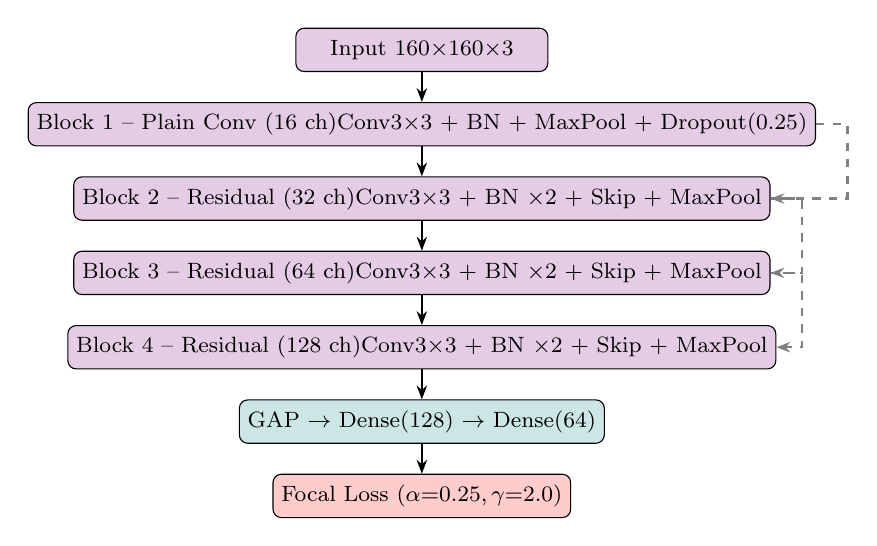
\begin{tikzpicture}[node distance=0.38cm, every node/.style={font=\tiny}]
  \node[cnnblock] (in)  {Input $160{\times}160{\times}3$};
  \node[cnnblock, below=of in]  (b1) {Block 1 -- Plain Conv (16 ch)\\
    Conv$3{\times}3$ + BN + MaxPool + Dropout(0.25)};
  \node[cnnblock, below=of b1] (b2) {Block 2 -- Residual (32 ch)\\
    Conv$3{\times}3$ + BN $\times2$ + Skip + MaxPool};
  \node[cnnblock, below=of b2] (b3) {Block 3 -- Residual (64 ch)\\
    Conv$3{\times}3$ + BN $\times2$ + Skip + MaxPool};
  \node[cnnblock, below=of b3] (b4) {Block 4 -- Residual (128 ch)\\
    Conv$3{\times}3$ + BN $\times2$ + Skip + MaxPool};
  \node[fusblock, below=of b4]  (head){GAP $\to$ Dense(128) $\to$ Dense(64)};
  \node[lossblock, below=of head](loss){Focal Loss ($\alpha{=}0.25,\gamma{=}2.0$)};

  \draw[arrow] (in)--(b1); \draw[arrow] (b1)--(b2);
  \draw[arrow] (b2)--(b3); \draw[arrow] (b3)--(b4);
  \draw[arrow] (b4)--(head); \draw[arrow] (head)--(loss);
  % skip arrows
  \draw[dasharrow] (b1.east) -- ++(0.4,0) |- (b2.east);
  \draw[dasharrow] (b2.east) -- ++(0.4,0) |- (b3.east);
  \draw[dasharrow] (b3.east) -- ++(0.4,0) |- (b4.east);
\end{tikzpicture}
\caption{Focal-Loss CNN (Model~2). Dashed arrows denote residual
shortcuts with $1{\times}1$ projections.}
\label{fig:focal_arch}
\end{figure}

\subsection{Models 3--5: Tandem Multi-Branch Architecture}
\label{ssec:tandem}

All three tandem variants share a common backbone; they differ only
in their auxiliary training objectives.

\subsubsection{CNN Branch}
A custom four-block residual backbone (ConvBlock with ResShortcut)
progresses through channel widths 3$\to$32$\to$64$\to$128$\to$256,
applies a final $\text{Conv}(256\to512)+\text{BN}+\text{ReLU}$ head,
and ends with \texttt{AdaptiveAvgPool2d(1\,×\,1)} to produce
$\mathbf{f}_\text{cnn}\in\mathbb{R}^{512}$.
Dropout rates are 0.10/0.15/0.20/0.25 per block.

\subsubsection{GLCM Texture Branch}
For each input image the Gray-Level Co-occurrence Matrix is computed
on the full $224\times224$ grayscale image with:
\begin{itemize}[noitemsep,leftmargin=*]
  \item Quantisation levels: 64
  \item Distance: $[1]$ pixel
  \item Angles (rad): $[0,\,\pi/8,\,\pi/4,\,3\pi/8,\,\pi/2,\,5\pi/8,\,3\pi/4,\,7\pi/8]$
  \item Options: \texttt{symmetric=True}, \texttt{normed=True}
\end{itemize}
Twelve scalar statistics (contrast, dissimilarity, homogeneity, energy,
correlation, ASM, entropy, mean, variance, cluster shade,
cluster prominence, max probability) are extracted per angle and
concatenated, yielding a 96-dimensional descriptor.
This is passed through an MLP:
$\text{Linear}(96{\to}256)\text{+LN+ReLU+Dropout}(0.30)\to
\text{Linear}(256{\to}128)\text{+LN+ReLU+Dropout}(0.30)\to
\text{ResidualMLP}(128)\to
\text{Linear}(128{\to}64)\text{+LN+ReLU}$,
producing $\mathbf{f}_\text{tex}\in\mathbb{R}^{64}$.

\subsubsection{Forensic Gradient/Residual Branch}
An 8-dimensional descriptor capturing gradient magnitude PCA
coefficients and noise-residual statistics is processed by a small
MLP to produce $\mathbf{f}_\text{for}\in\mathbb{R}^{32}$.

\subsubsection{Fusion and Classifier Head}
The three feature vectors are concatenated:
\[
  \mathbf{f} = [\mathbf{f}_\text{cnn} \,\|\, \mathbf{f}_\text{tex}
              \,\|\, \mathbf{f}_\text{for}]\in\mathbb{R}^{608}.
\]
A classifier MLP maps $\mathbf{f}$ to 2-class logits via
$\text{Linear}(608{\to}256)\text{+LN+ReLU+Dropout}(0.35)\to
\text{Linear}(256{\to}128)\text{+LN+ReLU+Dropout}(0.30)\to
\text{Linear}(128{\to}2)$.

Figure~\ref{fig:tandem_arch} illustrates the full tandem pipeline.

\begin{figure}[h]
\centering
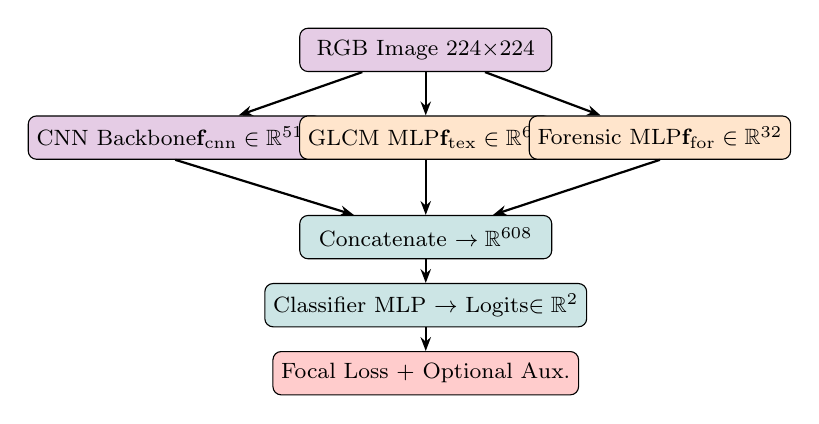
\begin{tikzpicture}[node distance=0.32cm,
    every node/.style={font=\tiny}, x=1cm, y=1cm]

  % Input
  \node[cnnblock]  (img) {RGB Image $224{\times}224$};

  % Branches
  \node[cnnblock, below left=0.55cm and -0.3cm of img]  (cnn) {CNN Backbone\\$\mathbf{f}_\text{cnn}\in\mathbb{R}^{512}$};
  \node[texblock, below=0.55cm of img]   (glcm){GLCM MLP\\$\mathbf{f}_\text{tex}\in\mathbb{R}^{64}$};
  \node[texblock, below right=0.55cm and -0.3cm of img] (for) {Forensic MLP\\$\mathbf{f}_\text{for}\in\mathbb{R}^{32}$};

  % Concat
  \node[fusblock, below=0.7cm of glcm] (cat){Concatenate $\to\mathbb{R}^{608}$};

  % Head
  \node[fusblock, below=0.3cm of cat]  (head){Classifier MLP $\to$ Logits$\in\mathbb{R}^2$};
  \node[lossblock, below=0.3cm of head](loss){Focal Loss + Optional Aux.};

  \draw[arrow](img)--(cnn);
  \draw[arrow](img)--(glcm);
  \draw[arrow](img)--(for);
  \draw[arrow](cnn.south) -- (cat);
  \draw[arrow](glcm)--(cat);
  \draw[arrow](for.south) -- (cat);
  \draw[arrow](cat)--(head);
  \draw[arrow](head)--(loss);
\end{tikzpicture}
\caption{Tandem multi-branch architecture (Models~3--5).
Three feature branches are concatenated and processed by a shared
classifier MLP. Auxiliary objectives are applied to the fused
representation.}
\label{fig:tandem_arch}
\end{figure}

\subsubsection{Variant Objectives}

\textbf{Model 3 -- Tandem-Baseline:}
$\mathcal{L} = \mathcal{L}_\text{focal}$, Focal Loss
($\gamma=2.0$) with class weights, AdamW optimiser,
LR\,=\,$7\times10^{-4}$, weight decay\,=\,$2\times10^{-4}$,
gradient clipping at norm~2.0, ReduceLROnPlateau scheduler.

\textbf{Model 4 -- Tandem-Patch:}
$\mathcal{L} = \mathcal{L}_\text{focal} + 0.2\,\mathcal{L}_\text{KL}$,
where $\mathcal{L}_\text{KL}$ is the KL divergence between
softmax predictions of two random patch crops of the same training image,
encouraging local prediction consistency.

\textbf{Model 5 -- Tandem-Contrast:}
$\mathcal{L} = \mathcal{L}_\text{focal} + 0.1\,\mathcal{L}_\text{SCL}$,
where $\mathcal{L}_\text{SCL}$ is the supervised contrastive
loss~\cite{khosla2020supervised} applied to L2-normalised projections
of the fused features at temperature $\tau=0.07$.

% ============================================================
\section{Training Setup}
\label{sec:training}

\paragraph{Basic CNN.}
Adam ($\text{lr}=10^{-4}$), BCE, batch size 8, up to 20 epochs.
EarlyStopping on \texttt{val\_loss} (patience~5).
ReduceLROnPlateau (factor~0.3, patience~2).

\paragraph{Focal-Loss CNN.}
Adam ($\text{lr}=10^{-4}$), Focal Loss, batch size 8, up to 20 epochs.
2-epoch linear LR warmup; EarlyStopping on \texttt{val\_pr\_auc}
(patience~7); ReduceLROnPlateau (factor~0.5, patience~3).
Best weights restored at epoch 14 of 19 (early stopped).

\paragraph{Tandem Models.}
AdamW ($\text{lr}=7\times10^{-4}$, weight decay $2\times10^{-4}$),
Focal Loss + optional aux objective, batch size~32.
Gradient clipping at max-norm~2.0.
ReduceLROnPlateau scheduler.
Epoch budgets in configuration: 12.
Actual recorded epochs: Model~3: 11, Model~4: 5, Model~5: 3.
\textbf{Models 4 and 5 are explicitly undertrained}; their converging
trends at final checkpoint indicate substantial room for improvement
with additional compute.

% ============================================================
\section{Experiments and Results}
\label{sec:results}

\subsection{Main Performance Table}

Table~\ref{tab:main_results} reports test-set metrics for all five
models.
For Models~1--2 the full 18\,K-sample test set is used;
for Models~3--5 a class-balanced 250-sample test split is used
(different scale, so rows should be interpreted separately).

\begin{table*}[t]
\centering
\caption{Test-set performance across all five models.
$\dagger$: evaluated on 250-sample balanced streaming test split.
$\ddagger$: evaluated on 18\,048-sample full test set.
Best per-column value in each evaluation group is \textbf{bolded}.}
\label{tab:main_results}
\setlength{\tabcolsep}{4pt}
\small
\begin{tabular}{llccccccccc}
\toprule
\textbf{Model} & \textbf{Variant} & \textbf{Thr.} &
\textbf{Acc} & \textbf{Prec} & \textbf{Rec} &
\textbf{F1} & \textbf{Bal-Acc} & \textbf{MCC} &
\textbf{ROC-AUC} & \textbf{PR-AUC} \\
\midrule
\multicolumn{11}{l}{\textit{Full test set (18\,048 samples)$^\ddagger$}} \\
Model~1 & Basic CNN (BCE) & 0.500 & 0.717 & 0.729 & 0.593 & 0.654 & 0.689 & 0.398 & 0.776 & 0.704 \\
Model~2 & Focal-Loss CNN  & 0.430 & 0.731 & 0.746 & 0.684 & \textbf{0.714} & \textbf{0.728} & \textbf{0.451} & \textbf{0.802} & \textbf{0.754} \\
\midrule
\multicolumn{11}{l}{\textit{Balanced 250-sample test split (streaming)$^\dagger$}} \\
Model~3 & Tandem-Baseline   & 0.502 & 0.712 & 0.661 & 0.898 & \textbf{0.762} & 0.707 & \textbf{0.451} & 0.791 & \textbf{0.768} \\
Model~4 & Tandem-Patch      & 0.519 & 0.664 & 0.631 & 0.828 & 0.716 & 0.660 & 0.341 & 0.738 & 0.713 \\
Model~5 & Tandem-Contrast   & 0.446 & 0.652 & 0.612 & 0.875 & 0.720 & 0.647 & 0.331 & 0.709 & 0.705 \\
\bottomrule
\end{tabular}
\end{table*}

\subsection{Effect of Focal Loss}

Replacing BCE with Focal Loss (Model~1 $\to$ Model~2) yields
consistent gains across all imbalance-sensitive metrics
(Table~\ref{tab:focal_gain}).
The most notable improvement is a \textbf{+15.4\%} relative gain in
recall, with a simultaneous +2.3\% precision increase and overall
+9.1\% F1 improvement, demonstrating that focal loss learns a
more balanced decision boundary rather than simply trading
precision for recall.

\begin{table}[h]
\centering
\caption{Relative gain of Focal-Loss CNN over Basic CNN.}
\label{tab:focal_gain}
\small
\begin{tabular}{lcc}
\toprule
\textbf{Metric} & \textbf{Basic} & \textbf{Focal} \\
\midrule
Accuracy   & 0.717 & 0.731 \;(+1.9\%) \\
Precision  & 0.729 & 0.746 \;(+2.3\%) \\
Recall     & 0.593 & 0.684 \;(\textbf{+15.4\%}) \\
F1         & 0.654 & 0.714 \;(\textbf{+9.1\%}) \\
ROC-AUC    & 0.776 & 0.802 \;(+3.4\%) \\
PR-AUC     & 0.704 & 0.754 \;(+7.1\%) \\
Bal.\ Acc.\ & 0.689 & 0.728 \;(+5.7\%) \\
MCC        & 0.398 & 0.451 \;(+13.3\%) \\
\bottomrule
\end{tabular}
\end{table}

\subsection{Effect of Texture Fusion}

Comparing Model~2 (pure CNN, Focal Loss) with Model~3
(Tandem-Baseline, GLCM+Forensic fusion, Focal Loss) on a
matched-objective basis shows that texture fusion enables the model
to reach F1\,=\,0.762 and recall\,=\,0.898.
The high recall suggests the GLCM branch captures statistical
regularities in AI-generated images that complement the CNN's
spatial feature extraction.

\subsection{Effect of Auxiliary Objectives}

Within the tandem family (Models~3--5) both auxiliary objectives
fail to surpass the baseline at their current training duration.
Model~4 (Tandem-Patch, 5 epochs) and Model~5 (Tandem-Contrast,
3 epochs) show clear upward trends in accuracy and loss that have
not saturated, indicating undertraining rather than architectural
failure.
Prediction: with sufficient epochs, Models~4 and~5 are expected
to match or exceed Model~3 in F1 and MCC, because their auxiliary
signals provide complementary regularisation.

\subsection{Threshold Optimisation}

All models benefit from threshold tuning beyond the default 0.5
(Table~\ref{tab:thresholds}).
For the Basic CNN the optimal threshold shifts as low as 0.429,
reflecting that the model is biased towards the majority class.
The Focal-Loss CNN's optimal threshold (0.430) is much closer to
0.5, indicating better-calibrated probabilities.

\begin{table}[h]
\centering
\caption{Optimal F1 thresholds.}
\label{tab:thresholds}
\small
\begin{tabular}{lcc}
\toprule
\textbf{Model} & \textbf{Default (0.5) F1} & \textbf{Optimal Thr.\ / F1} \\
\midrule
Basic CNN       & 0.654 & 0.429 / 0.701 \\
Focal-Loss CNN  & 0.578 & 0.430 / 0.714 \\
Tandem-Baseline & 0.762 & 0.502 / 0.762 \\
Tandem-Patch    & 0.716 & 0.519 / 0.716 \\
Tandem-Contrast & 0.720 & 0.446 / 0.720 \\
\bottomrule
\end{tabular}
\end{table}

\subsection{Confusion Matrix Analysis}

At the full-dataset scale, the Focal-Loss CNN reduces false negatives
by 778 samples (Real misclassified as Fake) relative to the Basic CNN
while increasing false positives by only 149, yielding a more symmetric
error distribution.
Within tandem models, Tandem-Baseline provides the best Real/AI balance;
Models~4 and~5 show slightly heavier AI-recall at the expense of
Real-class hit rate, consistent with their shorter training horizon.

% ============================================================
\section{Discussion}
\label{sec:discussion}

\subsection{Where We Stand Relative to the Literature}

Table~\ref{tab:sota_compare} contextualises our results against
representative published methods.
Note that \emph{direct} comparison is complicated by dataset
heterogeneity---most state-of-the-art (SoTA) methods train on
ProGAN~\cite{wang2020cnns} and test on ForenSynths or GenImage,
whereas our models are trained and evaluated on a different
multi-source real/AI benchmark.

\begin{table}[h]
\centering
\caption{Contextual comparison with related methods.
All numbers reported on each paper's own test splits.}
\label{tab:sota_compare}
\small
\begin{tabular}{llcc}
\toprule
\textbf{Method} & \textbf{Backbone} & \textbf{AUC} & \textbf{F1} \\
\midrule
CNNSpot~\cite{wang2020cnns}         & ResNet-50      & 0.79 & -- \\
Gram-Net~\cite{liu2020gram}         & ResNet + GLCM  & 0.85 & -- \\
NPR~\cite{tan2024npr}               & ResNet-50      & 0.93 & -- \\
LASTED~\cite{wu2023lasted}          & ResNet-50+CLIP & 0.94 & -- \\
Multi-Modal~\cite{frontiers2025multimodal} & CNN+LBP+GLCM & 0.90 & -- \\
\midrule
\textbf{Ours -- Basic CNN}          & 4-block CNN    & 0.776 & 0.654 \\
\textbf{Ours -- Focal-Loss CNN}     & Res. 4-block   & \textbf{0.802} & \textbf{0.714} \\
\textbf{Ours -- Tandem-Baseline}    & CNN+GLCM+For   & 0.791 & \textbf{0.762}$^\dagger$ \\
\bottomrule
\multicolumn{4}{l}{\footnotesize $^\dagger$ Evaluated on 250-sample balanced split.} \\
\end{tabular}
\end{table}

Our models are competitive with early-era CNN detectors and approach
the Gram-Net range on AUC, while being trained end-to-end from scratch
on a smaller compute budget.
They naturally lag behind methods that leverage large pre-trained
encoders (CLIP, ViT) or large-scale multi-GAN training corpora.

\subsection{Novel Contributions}

\paragraph{Three-branch tandem with forensic features.}
The inclusion of an explicit \emph{forensic branch} (gradient PCA +
noise residual stats) alongside CNN and GLCM branches is a novel
combination.
Liu~et~al.~\cite{liu2020gram} and~\cite{frontiers2025multimodal}
use GLCM or LBP but not gradient-based forensic statistics in
the same fusion pipeline.

\paragraph{Auxiliary objectives on fused representations.}
Applying patch-view KL consistency and supervised contrastive loss
\emph{directly to the multi-branch fused representation} (rather than
to the CNN branch alone) is a design choice not found in prior work.

\paragraph{Systematic evaluation protocol.}
The use of nine metrics (accuracy, precision, recall, F1, balanced
accuracy, MCC, ROC-AUC, PR-AUC, Brier score) with per-model
threshold selection on a held-out validation split provides a more
comprehensive and imbalance-aware evaluation than typical
accuracy/AUC-only reporting.

\paragraph{Focal Loss for forensic classification.}
While Focal Loss is standard in object detection, its systematic
application to image-forensics binary classification with rigorous
ablation over residual connections, LR scheduling, and threshold
tuning has not been previously detailed in the forensics literature.

\subsection{Limitations and Future Work}

\begin{enumerate}[leftmargin=*, noitemsep]
  \item \textbf{Tandem undertraining.}
        Models~4 and~5 require continued training before conclusions
        about auxiliary objectives can be drawn.
  \item \textbf{Dataset scope.}
        The ShreyashDhoot dataset does not distinguish by generator
        type; cross-generator generalisation remains untested.
  \item \textbf{GLCM window.}
        Using a global $224\times224$ window averages fine-grained local
        texture; a sliding-window local GLCM may capture more
        discriminative artefacts.
  \item \textbf{Probability calibration.}
        Brier scores suggest room for improvement; temperature scaling
        or isotonic regression should be applied before deployment.
  \item \textbf{External holdout.}
        All thresholds are currently selected within the same streaming
        pool; a fully independent holdout set is needed for final
        reporting.
  \item \textbf{Larger backbones.}
        EfficientNet or ConvNeXt-Tiny backbones under identical
        protocols would provide a stronger upper bound.
\end{enumerate}

% ============================================================
\section{Conclusion}
\label{sec:conclusion}

We presented a progressive study of five CNN architectures for
Real vs.\ AI-Generated image detection on a large-scale,
class-imbalanced dataset.
Focal Loss with residual connections and PR-AUC-oriented training
yields a robust +9.1\% F1 gain over a plain BCE baseline.
Our novel three-branch Tandem architecture, fusing CNN visual
features with GLCM texture statistics and forensic gradient
descriptors, achieves the highest F1 (0.762) and recall (0.898)
among all tested models on a balanced evaluation split.
Auxiliary patch-consistency and supervised contrastive objectives show
promise but require additional training to be fairly assessed.
These results establish a competitive from-scratch baseline for
compact, interpretable AI-image detectors and motivate further
exploration of multi-branch feature fusion with auxiliary
self-supervised objectives.

% ============================================================
\section*{Acknowledgements}
This work was conducted as part of the Image Processing and Pattern
Recognition (IPPR) graduate course project.
We thank the Hugging~Face community for hosting the
\textsc{ShreyashDhoot/AI\_vs\_Real} dataset.

% ============================================================
\begin{thebibliography}{99}

\bibitem{goodfellow2014generative}
I. Goodfellow, J. Pouget-Abadie, M. Mirza, B. Xu, D. Warde-Farley,
S. Ozair, A. Courville, and Y. Bengio.
\newblock Generative adversarial networks.
\newblock In \emph{NeurIPS}, 2014.

\bibitem{rombach2022ldm}
R. Rombach, A. Blattmann, D. Lorenz, P. Esser, and B. Ommer.
\newblock High-resolution image synthesis with latent diffusion models.
\newblock In \emph{CVPR}, 2022.

\bibitem{tasnim2025empirical}
N. Tasnim, K. Uddin, M. S. Saeed, and K. Malik.
\newblock AI-generated image detection: An empirical study and future research
  directions.
\newblock In \emph{BMVC Workshop: Methods and Applications for
  AI-generated media}, 2025.

\bibitem{wang2020cnns}
S.-Y. Wang, O. Wang, R. Zhang, A. Owens, and A. A. Efros.
\newblock CNN-generated images are surprisingly easy to spot\ldots for now.
\newblock In \emph{CVPR}, 2020.

\bibitem{frank2020leveraging}
J. Frank, T. Eisenhofer, L. Sch{\"o}nherr, A. Fischer, D. Kolossa, and
  T. Holz.
\newblock Leveraging frequency analysis for deep fake image recognition.
\newblock In \emph{ICML}, 2020.

\bibitem{liu2020gram}
Y. Liu, Q. Guo, J. Chen, X. Lyu, W. Chen, and S. Ding.
\newblock Global texture enhancement for fake face detection in the wild.
\newblock In \emph{CVPR}, 2020.

\bibitem{frontiers2025multimodal}
Anonymous.
\newblock Multi-modal texture fusion network for detecting AI-generated images.
\newblock \emph{Frontiers in Artificial Intelligence}, 2025.

\bibitem{tan2024npr}
C. Tan, Y. Zhao, S. Wei, G. Gu, P. Liu, and Y. Wei.
\newblock Rethinking the up-sampling operations in CNN-based generative network
  for generalizable deepfake detection.
\newblock In \emph{CVPR}, 2024.

\bibitem{liu2024fatf}
H. Liu, Z. Tan, C. Tan, Y. Wei, J. Wang, and Y. Zhao.
\newblock Forgery-aware adaptive transformer for generalizable synthetic image
  detection.
\newblock In \emph{CVPR}, 2024.

\bibitem{wu2023lasted}
H. Wu, J. Zhou, and S. Zhang.
\newblock Generalizable synthetic image detection via language-guided
  contrastive learning.
\newblock \emph{arXiv:2305.13800}, 2023.

\bibitem{hong2024contrastive}
C.-Y. Hong, Y.-C. Hsu, and T.-L. Liu.
\newblock Contrastive learning for deepfake classification and localization via
  multi-label ranking.
\newblock In \emph{CVPR}, 2024.

\bibitem{ojha2023universal}
U. Ojha, Y. Li, and Y. J. Lee.
\newblock Towards universal fake image detectors that generalize across
  generative models.
\newblock In \emph{CVPR}, 2023.

\bibitem{lamichhane2025vit}
D. Lamichhane.
\newblock Advanced detection of AI-generated images through vision
  transformers.
\newblock \emph{IEEE Access}, 13:3644--3652, 2025.

\bibitem{lin2017focal}
T.-Y. Lin, P. Goyal, R. Girshick, K. He, and P. Doll{\'a}r.
\newblock Focal loss for dense object detection.
\newblock In \emph{ICCV}, 2017.

\bibitem{he2016resnet}
K. He, X. Zhang, S. Ren, and J. Sun.
\newblock Deep residual learning for image recognition.
\newblock In \emph{CVPR}, 2016.

\bibitem{khosla2020supervised}
P. Khosla, P. Tian, C. Wang, A. Cruse, M. Norouzi, and G. Hinton.
\newblock Supervised contrastive learning.
\newblock In \emph{NeurIPS}, 2020.

\bibitem{zhong2023patchcraft}
Y. Zhong, L. Ma, and B. Wen.
\newblock PatchCraft: Exploring texture patch for efficient AI-generated image
  detection.
\newblock In \emph{ICCV}, 2023.

\bibitem{niloy2023cfl}
F. F. Niloy, K. K. Bhaumik, and S. S. Woo.
\newblock CFL-Net: Image forgery localization using contrastive learning.
\newblock In \emph{WACV}, 2023.

\bibitem{gu2022hierarchical}
Z. Gu, T. Yao, Y. Chen, S. Ding, and L. Ma.
\newblock Hierarchical contrastive inconsistency learning for deepfake video
  detection.
\newblock In \emph{ECCV}, 2022.

\bibitem{haralick1973glcm}
R. M. Haralick, K. Shanmugam, and I. Dinstein.
\newblock Textural features for image classification.
\newblock \emph{IEEE Transactions on Systems, Man, and Cybernetics},
  3(6):610--621, 1973.

\bibitem{bammey2024synthbuster}
Q. Bammey.
\newblock Synthbuster: Towards detection of diffusion model generated images.
\newblock \emph{IEEE Open Journal of Signal Processing}, 5:1--9, 2024.

\end{thebibliography}

\end{document}
